%  Template for ICASSP-2021 paper; to be used with:
%          spconf.sty  - ICASSP/ICIP LaTeX style file, and
%          IEEEbib.bst - IEEE bibliography style file.
% --------------------------------------------------------------------------
\documentclass{article}
\usepackage{spconf,amsmath,graphicx,hyperref}

% Example definitions.
% --------------------
\def\x{{\mathbf x}}
\def\L{{\cal L}}

% Title.
% ------
\title{AIML 425 Project}
%
% Single address.
% ---------------
\name{Quan Zhao (Student ID: 300471028)}
%\name{Author(s) Name(s)\thanks{Thanks to XYZ agency for funding.}}
\address{Victoria University of Wellington}


\begin{document}
%\ninept
%
\maketitle
%
\section{Introduction}
\label{sec:intro}

Face Detection stands at the forefront of research, given its myriad applications across various industries. 
The advent of Neural Networks has revolutionized this domain, leading to the development of numerous sophisticated face detection algorithms. 
Among these, RetinaFace has emerged as a notable contender. 
Introduced in 2019 and subsequently accepted by the esteemed "Conference on Computer Vision and Pattern Recognition (CVPR)" in 2020, 
RetinaFace has garnered significant attention. 
This study delves into the intricacies of RetinaFace, 
drawing insights from the paper "RetinaFace: Single-shot Multi-level Face Localisation in the Wild" \cite{deng2020retinaface}. 
While the pretrained model of RetinaFace exhibits commendable performance, it's not without its limitations, 
especially when confronted with real-world edge cases. 
Retraining the entire model can be resource-intensive, prompting the exploration of fine-tuning as a viable alternative. 
This study aims to shed light on the fine-tuning approach, offering a pathway to optimize the model for specific applications.

\section{Content Analysis}
\label{sec:content}

In the paper "RetinaFace: Single-shot Multi-level Face Localisation in the Wild" \cite{deng2020retinaface}, the author presents a unique pixel-wise face localization method termed as RetinaFace. This innovative approach adopts a single-stage design and utilizes a multi-task learning strategy. Through this, it can concurrently predict diverse attributes associated with a face. In this section, we delve into the intricate details of the RetinaFace model and provide insights into its functioning.

\subsection{RetinaFace Overview}

Derived from its name, RetinaFace is an adaptation of the RetinaNet architecture, specifically tailored for face detection tasks. It primarily consists of three pivotal components: the Feature Pyramid Network (FPN), the Context Module, and Cascade Regression accompanied by a Multi-task Loss.

The high-level structure of the RetinaFace network is depicted in Fig~\ref{fig:structure}, which has been sourced from the original paper \cite{deng2020retinaface}.

\begin{figure}[h]
  \centering
  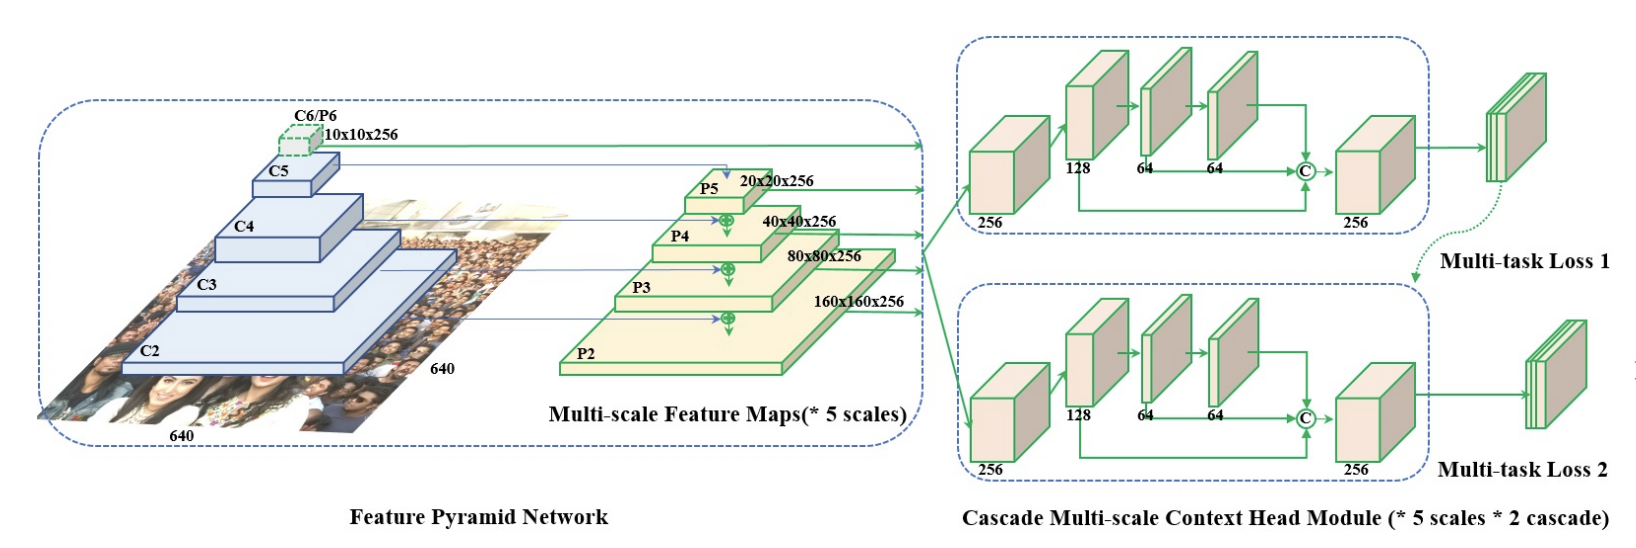
\includegraphics[width=0.7\linewidth]{images/network_structure}
  \caption{Network structure of RetinaFace.}
  \label{fig:structure}
\end{figure}

For the scope of this discussion, our primary emphasis will be on elucidating the face detection prowess of RetinaFace.

\subsection{Feature Pyramid Network (FPN)}

In the annals of computer vision, image pyramids have been quintessential for processing images across multiple scales to detect objects of different sizes. Deep convolutional neural networks (CNNs) inherently generate feature maps at varying resolutions. Specifically, shallow layers yield high-resolution features with weak semantic information, whereas deeper layers present a converse scenario: they offer rich semantic insights but at a compromised spatial resolution. The Feature Pyramid Network (FPN) \cite{lin2017feature} ingeniously taps into these multi-scale features to amplify object detection capabilities.

Within the architecture of FPN, there exists a \textbf{Bottom-up Pathway}, which is essentially the standard forward pass witnessed in CNNs. As one progresses deeper into this pathway, the semantic richness augments, but there's an accompanying sacrifice in spatial resolution.

Contrastingly, the FPN introduces a \textbf{Top-down Pathway} along with \textbf{Lateral Connections}. Here, there's a reversal in the operational flow—spatial resolution is upsampled. While this upsampling is in process, lateral connections, which originate from the bottom-up pathway, are seamlessly integrated. The confluence of these connections and the upsampled features results in a harmonized blend of high-level semantic knowledge and intricate spatial details.

One of the hallmarks of FPN is its prowess in \textbf{Multi-scale Predictions}. The network leverages the coalesced features across its pyramid structure, ensuring predictions are attuned to a myriad of scales. This equips FPN with a discerning eye, enabling it to adeptly identify objects regardless of their size.

The inception of FPN addressed and rectified some inherent limitations of traditional CNNs, particularly the challenges associated with detecting minuscule objects. By marrying the contrasting strengths of low-resolution, semantically charged features with their high-resolution, semantically impoverished counterparts, FPN delivers an enhanced detection spectrum across varying scales. A notable efficiency of FPN is its ability to sculpt a feature pyramid out of a single-scale input image, which accentuates computational efficiency.

Given its prowess and innovations, it's no surprise that FPN has found itself embedded as a foundational component in numerous state-of-the-art object detection architectures, including RetinaNet. Its innate ability to represent features across scales supercharges a detector's proficiency in recognizing objects spanning different sizes.

\begin{figure}[h]
  \centering
  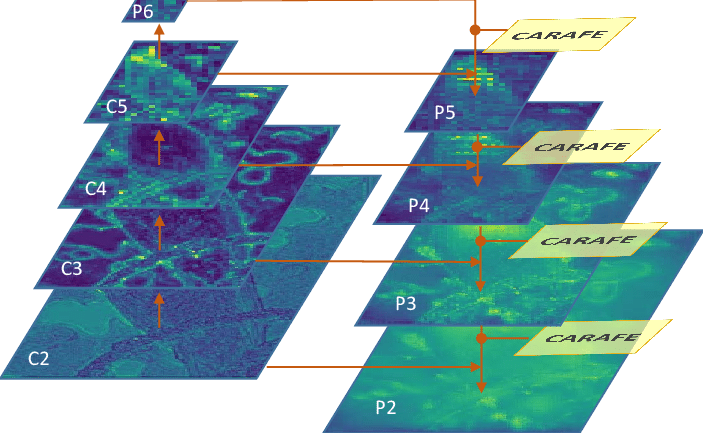
\includegraphics[width=0.7\linewidth]{images/fpn}
  \caption{Feature Pyramid Network (FPN) architecture}
  \label{fig:fpn}
\end{figure}

Figure~\ref{fig:fpn} illustrates the architecture of the Feature Pyramid Network (FPN), as delineated in prior works \cite{wang2019carafe}.

At its core, the Feature Pyramid Network (FPN) represents a groundbreaking evolution in object detection, 
adeptly tackling the challenges of multi-scale object detection. 

Through the adept fusion of multi-scale feature representations, FPN not only enhances the accuracy but also the operational efficiency of object detection mechanisms.

\subsubsection{Anchor-based Face Detection on Pyramid Network}

In RetinaFace, anchors are densely arranged across the feature maps of pyramid levels like P2. However, rather than predicting on a pixel-by-pixel basis, anchors correspond to spatial locations on the feature map, with their density governed by the stride of the pyramid level.

Each pyramid level's stride signifies the spatial resolution disparity between the original image and its feature map. For example, a stride of 4 for P2 implies each of its spatial locations corresponds to a 4x4 region in the original image. At each spatial location on a feature map, multiple anchors of varied scales and aspect ratios are positioned. This means that at a specific x,y location on P2, there exist multiple anchors, each differing in size or shape.

While anchors densely populate the feature map, they don't correspond to every pixel of the original image. They relate to the feature map's spatial locations. For instance, with P2's stride of 4, the first set of anchors might center at pixel (2,2) of the original image, with subsequent sets at pixels like (6,2), and so forth.

Despite not predicting for each pixel, the amalgamation of diverse scales and aspect ratios ensures comprehensive coverage of all potential objects. This dense arrangement, coupled with the anchors' varied dimensions, equips the model to detect faces of multiple sizes and orientations.

Figure~\ref{fig:anochor_tiling_1} provides a visual representation of how anchor sampling operates at varying strides, drawing upon the insights from prior research \cite{yan2019iou}. 
Meanwhile, Figure~\ref{fig:anochor_tiling_2} demonstrates the functionality of anchors on the feature map level or stage, as elucidated in the earlier work by \cite{vo2022review}.

\begin{figure}[h]
  \centering
  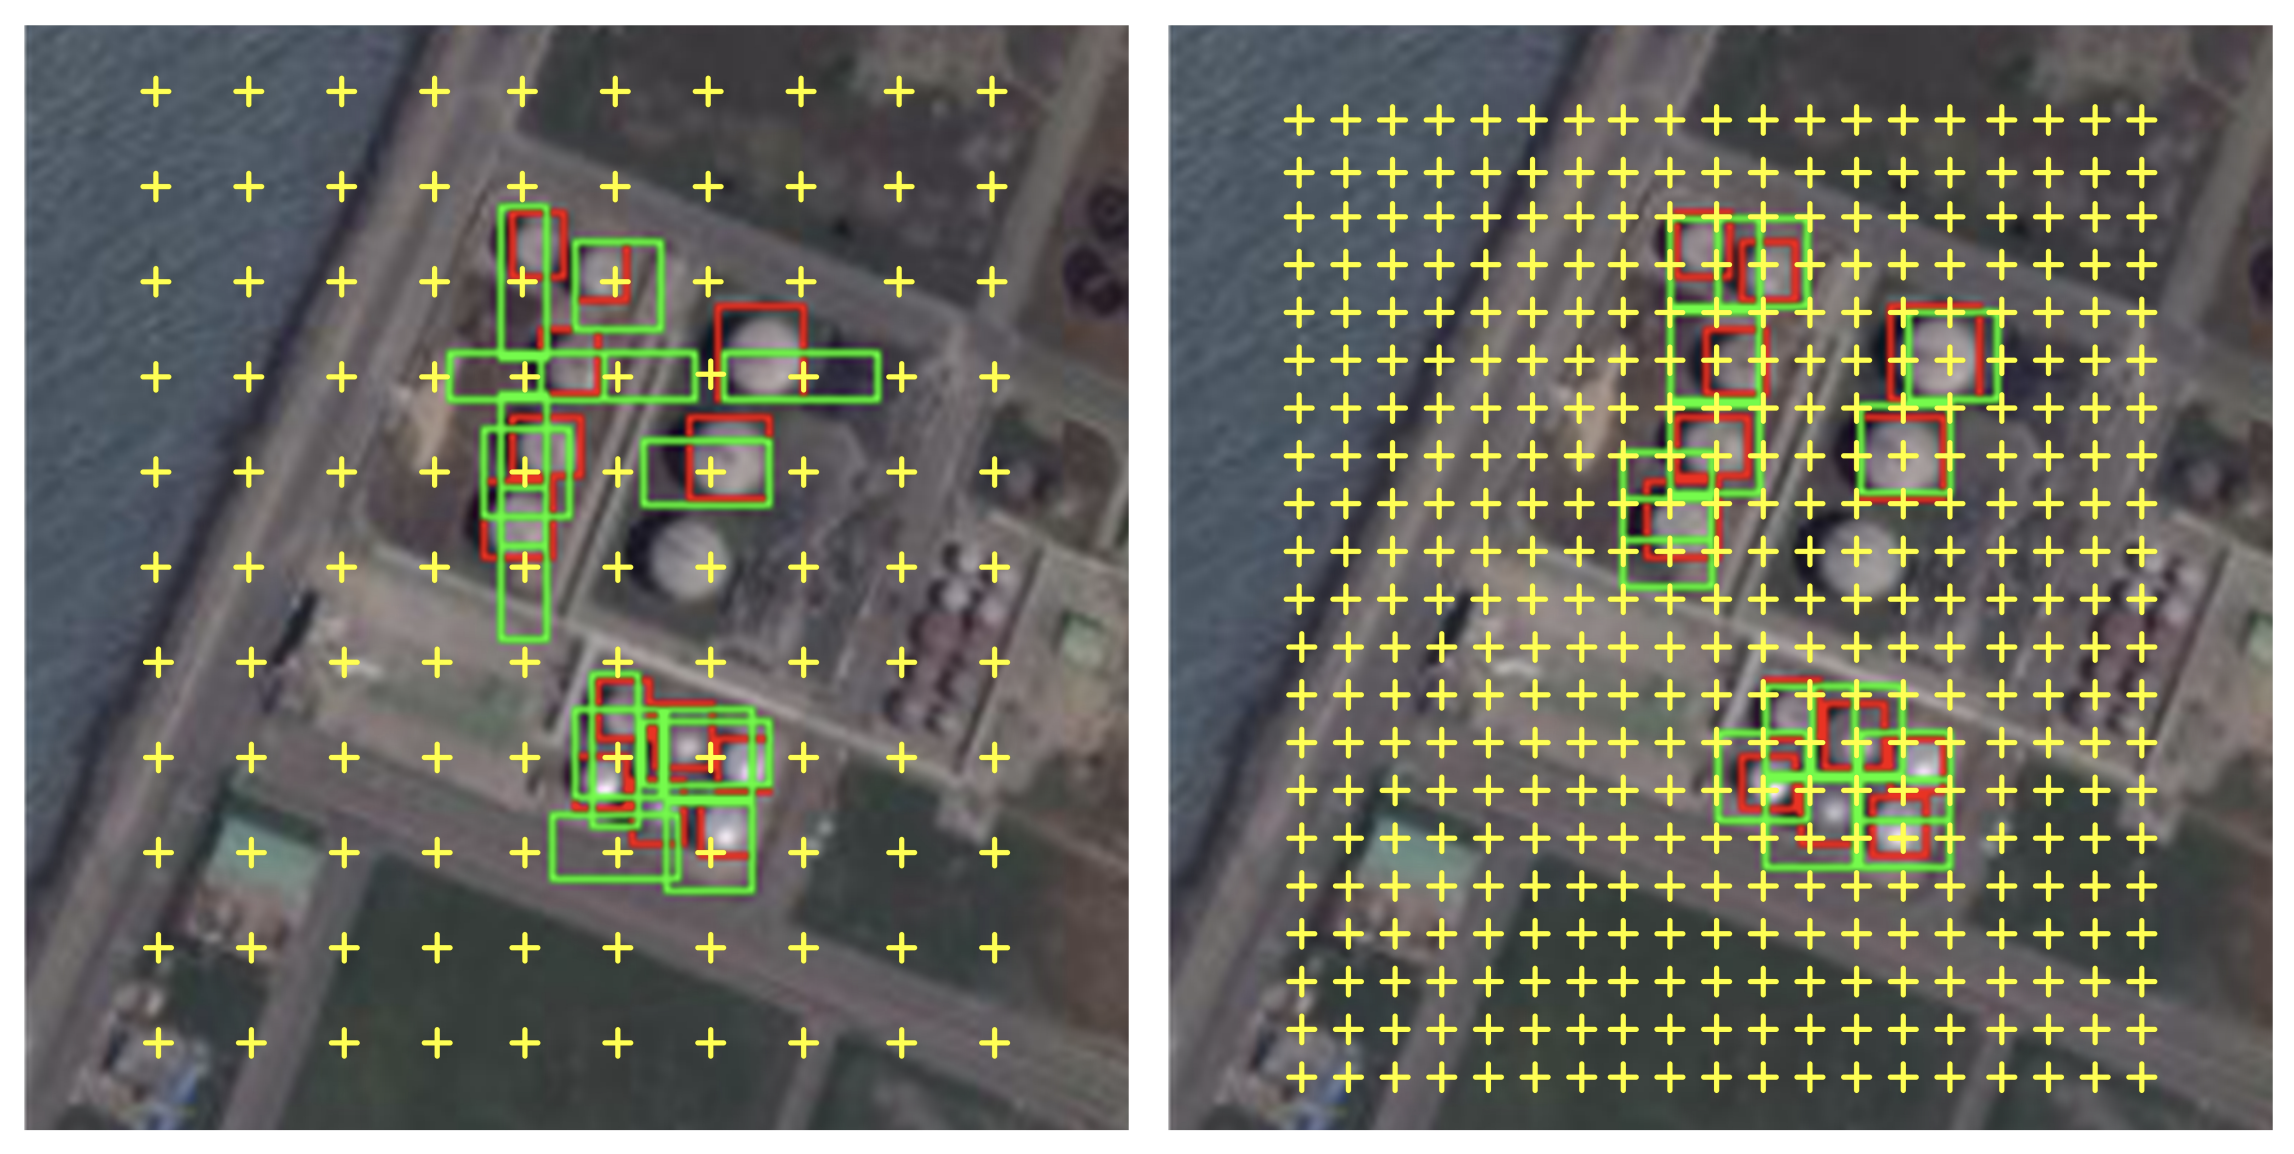
\includegraphics[width=0.7\linewidth]{images/anochor_tiling_1}
  \caption{Anchor sampling in different stride}
  \label{fig:anochor_tiling_1}
\end{figure}

\begin{figure}[h]
  \centering
  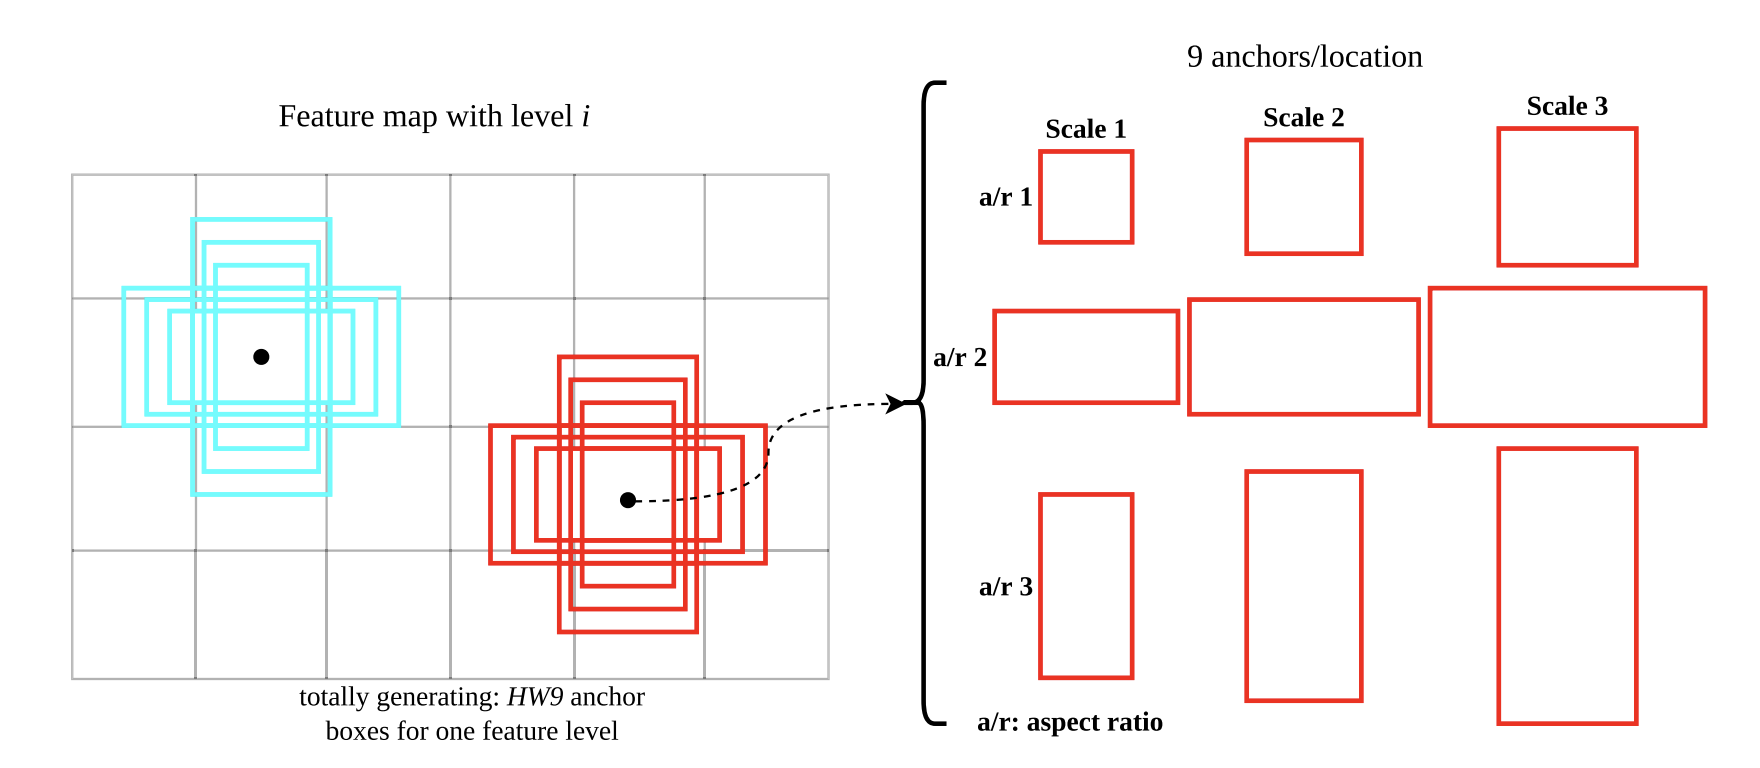
\includegraphics[width=0.7\linewidth]{images/anochor_tiling_2}
  \caption{Anchor box generator on the feature map with level i. The base anchor box has an area of $2^i$}
  \label{fig:anochor_tiling_2}
\end{figure}

In essence, RetinaFace's dense anchor tiling across pyramid feature maps doesn't operate on a strict pixel-by-pixel basis. Predictions are tethered to feature map spatial locations, with the density influenced by the pyramid level's stride.

\subsection{Context Module in RetinaFace}

The context module stands as a pivotal component within the RetinaFace architecture, designed to harness contextual information across various feature levels. Multi-level feature fusion, prevalent in many face detection architectures, is employed to cater to faces of diverse sizes and contexts. By aggregating context from different scales, the context module bolsters the feature representation, proving invaluable for detecting small faces or those in challenging scenarios where context offers crucial insights.

This module's integration results in enhanced detection performance, especially in situations with partial occlusions, varying face sizes, or challenging lighting. Essentially, the context module acts as a conduit to assimilate and capitalize on information from different scales, fortifying the RetinaFace detector's precision and robustness across varied real-world settings.

\subsubsection{How Context Module works with FPN}

The context module refines the multi-scale features furnished by the FPN by aggregating context, offering a dual enhancement. Initially, the FPN delivers multi-scale features, which the context module subsequently refines by integrating broader contextual data. This synergy between the FPN and the context module culminates in a richer feature representation for RetinaFace, making it more resilient and adept at face detection, particularly in demanding scenarios.

In a nutshell, while RetinaFace's FPN provides multi-scale feature representation, the context module further amplifies these features by incorporating contextual information, resulting in a potent face detection mechanism.

\subsection{Cascade Regression with Multi-task Loss}

Within RetinaFace, cascade regression refines bounding box predictions iteratively. While refining bounding boxes, the model concurrently optimizes other tasks using the multi-task loss, ensuring all tasks benefit from the iterative refinement. This amalgamation of cascade regression and multi-task loss enables the model to achieve precise bounding box predictions without sacrificing the performance of other tasks. In summary, the combination ensures iterative refinement of bounding box predictions, culminating in enhanced and consistent face detections.

\subsubsection{Cascade Regression}

Cascade regression in RetinaFace involves a series of regression operations for iterative bounding box refinement. Instead of a one-shot prediction, the model makes an initial bounding box prediction and refines it in subsequent stages. This iterative approach aims to yield more accurate and stable bounding box predictions, especially in challenging scenarios.

\subsubsection{Multi-task Loss}

RetinaFace's multi-task loss is crafted to manage multiple objectives concurrently, including face classification, bounding box regression, facial landmark regression, and dense regression. The loss function is given by:

\[ L = L_{cls}(p_i, p^*i) + \lambda_1 1{p^i} L*{box}(t_i, t^*i) \]
\[+ \lambda_2 1{p^i} L*{pts}(l_i, l^*i) + \lambda_3 1{p^i} L*{pixel} \]

Where \( 1_{p^*_i} \) is an indicator function (1 for positive anchors), and \( \lambda_1, \lambda_2, \lambda_3 \) are loss-balancing parameters. The loss components include face classification (\(L_{cls}\)), bounding box regression (\(L_{box}\)), facial landmark regression (\(L_{pts}\)), and dense regression (\(L_{pixel}\)).


\section{Impact}

The publication "RetinaFace: Single-shot Multi-level Face Localisation in the Wild" has left an indelible mark on face detection research, catalyzing numerous subsequent investigations.

\subsection{Improving the Architecture}
RetinaFace's architecture, while pivotal in human face detection, has seen adaptations for other species. For instance, \cite{xu2022cattlefacenet} introduced "CattleFaceNet: A cattle face identification approach based on RetinaFace and ArcFace loss," which melds RetinaFace's strengths with the ArcFace loss for enhanced cattle face recognition. Such innovative applications highlight the model's versatility across varied identification challenges.

\subsection{Adapting to Different Domains}
RetinaFace's adaptability shines in its applications across diverse scenarios. A pertinent example is \cite{aswal2020single}'s "Single Camera Masked Face Identification," addressing the complexities of identifying mask-obscured faces, a contemporary challenge. This underscores RetinaFace's ability to navigate domain-specific intricacies.

\subsection{Optimization for Real-time Applications}
Real-time face detection's importance, especially in constrained environments, has led to RetinaFace's optimization endeavors. \cite{putro2022faster}'s "A Faster Real-time Face Detector Support Smart Digital Advertising on Low-cost Computing Device" accentuates the model's significance in digital advertising on budget devices, underscoring its real-world applicability.

\subsection{Open-source Availability}

The generous decision by the authors to open-source both their code and models has had profound repercussions in the wider research landscape. By granting unrestricted access to their pioneering work, they inadvertently expedited the adoption rate and catalyzed a spate of research endeavors stemming from their foundational model.

This open-source ethos has not only democratized research access but also nurtured a spirit of collaboration within the research community. Researchers, both seasoned and nascent, have been able to dissect, understand, and build upon RetinaFace's intricacies. Consequently, this has led to the emergence of improved iterations, diverse applications, and enriched adaptations of the model. Such a communal approach has substantially bridged knowledge gaps and expedited advancements in face detection research.

\section{Fine tuning pretrained model}

Fine-tuning a pretrained face detection model entails tailoring a model—originally trained on a vast dataset—to accommodate a newer, often smaller, dataset. This approach becomes invaluable when confronted with a specialized dataset or application that deviates from the initial training context. In real-world scenarios, a pretrained model may struggle to encompass all possible environments. Challenges such as varied camera angles or distinct environmental conditions, like fog, further underscore the necessity for such fine-tuning.
\subsection{Fine-tuning with Frozen Early Layers}

Fine-tuning pretrained models on novel datasets is a prevalent strategy in deep learning, offering a balance between leveraging pre-existing knowledge and adapting to new data. A common approach during this process is to freeze the early layers of the model, allowing only the deeper layers to be updated. This section delves into the rationale behind this approach and its implications for model performance.

\subsubsection{Rationale for Freezing Early Layers}

\begin{enumerate}
\item Transfer of Generic Features: Deep neural networks, particularly convolutional architectures, have a hierarchical feature extraction process. The initial layers often capture universal, low-level features such as edges, textures, and colors. These foundational features are generally applicable across diverse datasets, making them valuable for transfer learning.

\item Mitigation of Overfitting: Fine-tuning all layers with a small novel dataset can lead to overfitting, where the model becomes overly specialized to the training data. By freezing the early layers, the number of trainable parameters is reduced, thus decreasing the model's capacity to overfit.

\item Computational Efficiency: Training fewer parameters can expedite the convergence of the model, leading to faster training epochs and potentially requiring fewer epochs to achieve optimal performance on the new dataset.
\end{enumerate}

\subsubsection{Why Freezing Early Layers Works?}
\begin{enumerate}
  \item Hierarchical Feature Learning: 
  
  As data progresses through the layers of a neural network, features transition from being generic to specific. 

Early layers often act as filters detecting fundamental patterns, while deeper layers combine these patterns to recognize more complex structures. 
When transferring to a new task, the basic patterns remain largely consistent, while the higher-level representations require adjustments to cater to the specifics of the new data.

\item Regularization Effect: 

By not allowing early layers to change, the model is implicitly regularized. This constraint can be viewed as a form of structural regularization, where certain parts of the model are kept constant, guiding the learning process in the deeper layers and preventing them from fitting to noise in the new dataset.

\item Data-driven Adaptation: 

While the early layers remain fixed, the deeper layers, which are more adaptable and data-specific, undergo training. This ensures that the model retains its generalization capability from the pretraining phase while fine-tuning based on the nuances of the new dataset.
\end{enumerate}

Freezing the early layers during fine-tuning strikes a balance between leveraging pre-existing, generic features and adapting to novel data characteristics. This approach, rooted in the hierarchical nature of feature extraction in deep networks, offers a computationally efficient and effective method for transfer learning across diverse tasks. Future research might explore adaptive freezing strategies, where the decision to freeze or train layers is data-driven, further optimizing the fine-tuning process.
  
\section{Experiment}

In this study, our experimental framework is rooted in the repository provided by \cite{biubug6_2020} on GitHub. We align our dataset with the renowned WIDER FACE benchmark \cite{yang2016wider}.

From the WIDER FACE dataset, we extracted three specific categories: ``Voter,'' ``Meeting,'' and ``People Marching'' to curate our specialized data. The initial approach entailed training the base model on the WIDER FACE dataset while consciously excluding these three categories. This model was then fine-tuned using data from only these three categories. We subsequently evaluated the adapted model's efficacy using an evaluation set from the same categories.

During the fine-tuning phase, we variably froze different layers of the model:

\begin{enumerate}
    \item \textbf{Experiment 1:} All layers were frozen, except for the head layers responsible for prediction.
    \item \textbf{Experiment 2:} All layers were frozen, excluding the head layers responsible for prediction and the backbone stage 1.
    \item \textbf{Experiment 3:} All layers were frozen, excluding the head layers responsible for prediction and the backbone stage 3.
\end{enumerate}

For each of these strategies, a rigorous cycle of hyperparameter optimization was undertaken, fine-tuning parameters like ``learning rates'', ``weight decays'', ``batch sizes'', and ``momentums''.

Upon analysis, the results indicated that Experiment 3 outperformed the other strategies, marking it as the most favorable among the three.

\section{Limitations and Future Works}

Our study faced constraints due to the extensive computational requirements of the fine-tuning, training, and evaluation processes. Given these limitations, we had a restricted opportunity to run our models multiple times, leading to the fine-tuned models not surpassing the base model in performance. As a result, our primary analysis revolves around comparing the outcomes among the modified models rather than against the base model.

Moving forward, there are avenues for potential improvements:
\begin{itemize}
    \item We aim to expand our range by experimenting with different layers to freeze and a broader spectrum of hyperparameters.
    \item Fine-tuning the model using varied anchor configurations presents another promising direction. While our current study didn't delve into this due to time constraints, future endeavors might focus on determining the optimal size and quantity of anchors. Leveraging clustering methodologies to ascertain these anchor configurations and subsequently updating the corresponding code might offer a novel avenue for enhancing the model's performance.
\end{itemize}

\section{CONCLUSION}
\label{sec:conclusion}

RetinaFace, an adaptation of the foundational RetinaNet architecture, has ushered in a new era of face detection. By leveraging the strengths of the Feature Pyramid Network (FPN) and integrating specialized components like the context module, RetinaFace offers a robust solution for detecting faces in diverse scenarios. The model's adaptability is further highlighted by its applications across various domains, from cattle identification to contemporary challenges like masked face detection.

Moreover, the potential for fine-tuning, whether through hyper-parameter adjustments or freezing early layers, allows RetinaFace to be tailored to specific datasets or applications. This balance between leveraging pre-existing knowledge and adapting to new data nuances underscores the model's versatility.

In essence, RetinaFace stands as a significant advancement in face detection, combining speed with accuracy. As the field continues to evolve, models like RetinaFace will undoubtedly serve as benchmarks, guiding future innovations in object detection.


\section{STATEMENT OF ALL TOOLS USED}
\label{sec:statementofalltoolsused}

In this study, the primary tool employed is \texttt{PyTorch}.

The source code associated with this project has been published on GitHub for public access. 
Interested readers can find the repository at the following link: \href{https://github.com/felixzhao/AIML425-Project}{GitHub Repository}. 
For detailed code contributions, please refer to the \texttt{README} within the repository.



% To start a new column (but not a new page) and help balance the last-page
% column length use \vfill\pagebreak.
% -------------------------------------------------------------------------
%\vfill
%\pagebreak

\vfill\pagebreak

% References should be produced using the bibtex program from suitable
% BiBTeX files (here: strings, refs, manuals). The IEEEbib.bst bibliography
% style file from IEEE produces unsorted bibliography list.
% -------------------------------------------------------------------------
\bibliographystyle{IEEEbib}
\bibliography{strings,refs}

\end{document}